% Options for packages loaded elsewhere
\PassOptionsToPackage{unicode}{hyperref}
\PassOptionsToPackage{hyphens}{url}
%
\documentclass[
  man,floatsintext]{apa6}
\usepackage{amsmath,amssymb}
\usepackage{lmodern}
\usepackage{iftex}
\ifPDFTeX
  \usepackage[T1]{fontenc}
  \usepackage[utf8]{inputenc}
  \usepackage{textcomp} % provide euro and other symbols
\else % if luatex or xetex
  \usepackage{unicode-math}
  \defaultfontfeatures{Scale=MatchLowercase}
  \defaultfontfeatures[\rmfamily]{Ligatures=TeX,Scale=1}
\fi
% Use upquote if available, for straight quotes in verbatim environments
\IfFileExists{upquote.sty}{\usepackage{upquote}}{}
\IfFileExists{microtype.sty}{% use microtype if available
  \usepackage[]{microtype}
  \UseMicrotypeSet[protrusion]{basicmath} % disable protrusion for tt fonts
}{}
\makeatletter
\@ifundefined{KOMAClassName}{% if non-KOMA class
  \IfFileExists{parskip.sty}{%
    \usepackage{parskip}
  }{% else
    \setlength{\parindent}{0pt}
    \setlength{\parskip}{6pt plus 2pt minus 1pt}}
}{% if KOMA class
  \KOMAoptions{parskip=half}}
\makeatother
\usepackage{xcolor}
\usepackage{graphicx}
\makeatletter
\def\maxwidth{\ifdim\Gin@nat@width>\linewidth\linewidth\else\Gin@nat@width\fi}
\def\maxheight{\ifdim\Gin@nat@height>\textheight\textheight\else\Gin@nat@height\fi}
\makeatother
% Scale images if necessary, so that they will not overflow the page
% margins by default, and it is still possible to overwrite the defaults
% using explicit options in \includegraphics[width, height, ...]{}
\setkeys{Gin}{width=\maxwidth,height=\maxheight,keepaspectratio}
% Set default figure placement to htbp
\makeatletter
\def\fps@figure{htbp}
\makeatother
\setlength{\emergencystretch}{3em} % prevent overfull lines
\providecommand{\tightlist}{%
  \setlength{\itemsep}{0pt}\setlength{\parskip}{0pt}}
\setcounter{secnumdepth}{-\maxdimen} % remove section numbering
% Make \paragraph and \subparagraph free-standing
\ifx\paragraph\undefined\else
  \let\oldparagraph\paragraph
  \renewcommand{\paragraph}[1]{\oldparagraph{#1}\mbox{}}
\fi
\ifx\subparagraph\undefined\else
  \let\oldsubparagraph\subparagraph
  \renewcommand{\subparagraph}[1]{\oldsubparagraph{#1}\mbox{}}
\fi
\newlength{\cslhangindent}
\setlength{\cslhangindent}{1.5em}
\newlength{\csllabelwidth}
\setlength{\csllabelwidth}{3em}
\newlength{\cslentryspacingunit} % times entry-spacing
\setlength{\cslentryspacingunit}{\parskip}
\newenvironment{CSLReferences}[2] % #1 hanging-ident, #2 entry spacing
 {% don't indent paragraphs
  \setlength{\parindent}{0pt}
  % turn on hanging indent if param 1 is 1
  \ifodd #1
  \let\oldpar\par
  \def\par{\hangindent=\cslhangindent\oldpar}
  \fi
  % set entry spacing
  \setlength{\parskip}{#2\cslentryspacingunit}
 }%
 {}
\usepackage{calc}
\newcommand{\CSLBlock}[1]{#1\hfill\break}
\newcommand{\CSLLeftMargin}[1]{\parbox[t]{\csllabelwidth}{#1}}
\newcommand{\CSLRightInline}[1]{\parbox[t]{\linewidth - \csllabelwidth}{#1}\break}
\newcommand{\CSLIndent}[1]{\hspace{\cslhangindent}#1}
\ifLuaTeX
\usepackage[bidi=basic]{babel}
\else
\usepackage[bidi=default]{babel}
\fi
\babelprovide[main,import]{english}
% get rid of language-specific shorthands (see #6817):
\let\LanguageShortHands\languageshorthands
\def\languageshorthands#1{}
% Manuscript styling
\usepackage{upgreek}
\captionsetup{font=singlespacing,justification=justified}

% Table formatting
\usepackage{longtable}
\usepackage{lscape}
% \usepackage[counterclockwise]{rotating}   % Landscape page setup for large tables
\usepackage{multirow}		% Table styling
\usepackage{tabularx}		% Control Column width
\usepackage[flushleft]{threeparttable}	% Allows for three part tables with a specified notes section
\usepackage{threeparttablex}            % Lets threeparttable work with longtable

% Create new environments so endfloat can handle them
% \newenvironment{ltable}
%   {\begin{landscape}\centering\begin{threeparttable}}
%   {\end{threeparttable}\end{landscape}}
\newenvironment{lltable}{\begin{landscape}\centering\begin{ThreePartTable}}{\end{ThreePartTable}\end{landscape}}

% Enables adjusting longtable caption width to table width
% Solution found at http://golatex.de/longtable-mit-caption-so-breit-wie-die-tabelle-t15767.html
\makeatletter
\newcommand\LastLTentrywidth{1em}
\newlength\longtablewidth
\setlength{\longtablewidth}{1in}
\newcommand{\getlongtablewidth}{\begingroup \ifcsname LT@\roman{LT@tables}\endcsname \global\longtablewidth=0pt \renewcommand{\LT@entry}[2]{\global\advance\longtablewidth by ##2\relax\gdef\LastLTentrywidth{##2}}\@nameuse{LT@\roman{LT@tables}} \fi \endgroup}

% \setlength{\parindent}{0.5in}
% \setlength{\parskip}{0pt plus 0pt minus 0pt}

% Overwrite redefinition of paragraph and subparagraph by the default LaTeX template
% See https://github.com/crsh/papaja/issues/292
\makeatletter
\renewcommand{\paragraph}{\@startsection{paragraph}{4}{\parindent}%
  {0\baselineskip \@plus 0.2ex \@minus 0.2ex}%
  {-1em}%
  {\normalfont\normalsize\bfseries\itshape\typesectitle}}

\renewcommand{\subparagraph}[1]{\@startsection{subparagraph}{5}{1em}%
  {0\baselineskip \@plus 0.2ex \@minus 0.2ex}%
  {-\z@\relax}%
  {\normalfont\normalsize\itshape\hspace{\parindent}{#1}\textit{\addperi}}{\relax}}
\makeatother

% \usepackage{etoolbox}
\makeatletter
\patchcmd{\HyOrg@maketitle}
  {\section{\normalfont\normalsize\abstractname}}
  {\section*{\normalfont\normalsize\abstractname}}
  {}{\typeout{Failed to patch abstract.}}
\patchcmd{\HyOrg@maketitle}
  {\section{\protect\normalfont{\@title}}}
  {\section*{\protect\normalfont{\@title}}}
  {}{\typeout{Failed to patch title.}}
\makeatother

\usepackage{xpatch}
\makeatletter
\xapptocmd\appendix
  {\xapptocmd\section
    {\addcontentsline{toc}{section}{\appendixname\ifoneappendix\else~\theappendix\fi\\: #1}}
    {}{\InnerPatchFailed}%
  }
{}{\PatchFailed}
\keywords{visual illusions, illusion game, Pyllusion, personality, general factor\newline\indent Word count: 5114}
\usepackage{lineno}

\linenumbers
\usepackage{csquotes}
\usepackage[titles]{tocloft}
\cftpagenumbersoff{figure}
\renewcommand{\cftfigpresnum}{\itshape\figurename\enspace}
\renewcommand{\cftfigaftersnum}{.\space}
\setlength{\cftfigindent}{0pt}
\setlength{\cftafterloftitleskip}{0pt}
\settowidth{\cftfignumwidth}{Figure 10.\qquad}
\usepackage[labelfont=bf, font={scriptsize, color=gray}]{caption}
\ifLuaTeX
  \usepackage{selnolig}  % disable illegal ligatures
\fi
\IfFileExists{bookmark.sty}{\usepackage{bookmark}}{\usepackage{hyperref}}
\IfFileExists{xurl.sty}{\usepackage{xurl}}{} % add URL line breaks if available
\urlstyle{same} % disable monospaced font for URLs
\hypersetup{
  pdftitle={Too Beautiful to be Fake: Attractive Faces are Less Likely to be Judged as Artificially Generated},
  pdfauthor={Dominique Makowski1, An Shu Te1, Stephanie Kirk1, Ngoi Zi Liang1, \& S.H. Annabel Chen1, 2, 3, 4},
  pdflang={en-EN},
  pdfkeywords={visual illusions, illusion game, Pyllusion, personality, general factor},
  hidelinks,
  pdfcreator={LaTeX via pandoc}}

\title{\textbf{Too Beautiful to be Fake: Attractive Faces are Less Likely to be Judged as Artificially Generated}}
\author{Dominique Makowski\textsuperscript{1}, An Shu Te\textsuperscript{1}, Stephanie Kirk\textsuperscript{1}, Ngoi Zi Liang\textsuperscript{1}, \& S.H. Annabel Chen\textsuperscript{1, 2, 3, 4}}
\date{}


\shorttitle{Illusion Game Validation}

\authornote{

Correspondence concerning this article should be addressed to Dominique Makowski, HSS 04-18, 48 Nanyang Avenue, Singapore (\href{mailto:dom.makowski@gmail.com}{\nolinkurl{dom.makowski@gmail.com}}).

The authors made the following contributions. Dominique Makowski: Conceptualization, Data curation, Formal Analysis, Funding acquisition, Investigation, Methodology, Project administration, Resources, Software, Supervision, Validation, Visualization, Writing -- original draft; An Shu Te: Project administration, Resources, Investigation, Writing -- original draft; Stephanie Kirk: Project administration, Resources, Writing -- original draft; Ngoi Zi Liang: Project administration, Resources, Writing -- review \& editing; S.H. Annabel Chen: Project administration, Supervision, Writing -- review \& editing.

Correspondence concerning this article should be addressed to Dominique Makowski, HSS 04-18, 48 Nanyang Avenue, Singapore. E-mail: \href{mailto:dom.makowski@gmail.com}{\nolinkurl{dom.makowski@gmail.com}}

}

\affiliation{\vspace{0.5cm}\textsuperscript{1} School of Social Sciences, Nanyang Technological University, Singapore\\\textsuperscript{2} LKC Medicine, Nanyang Technological University, Singapore\\\textsuperscript{3} National Institute of Education, Singapore\\\textsuperscript{4} Centre for Research and Development in Learning, Nanyang Technological University, Singapore}

\abstract{%
Abstract abstract abstract.
}



\begin{document}
\maketitle

For the first time in Humanity's history, technology has enabled the creation of near-perfect simulations indistinguishable from reality. These artificial yet realistic constructs permeate all areas of life through immersive works of fiction, deep fakes (real-like images and videos generated by deep learning algorithms), virtual and augmented reality, artificial beings (artificial intelligence ``bots'' with or without a physical form), fake news and skewed narratives which ground truth is often hard to access. They carry important consequences for the technological and entertainment sector, but also for security and politics, for instance if used for propaganda and disinformation, recruitment into malevolent organizations, or religious indoctrination. This challenge is central to what has been coined as the ``post-truth era'' (\textbf{REF Lewandowsky et al., 2017}), in which the distinction (and lack thereof) between authentic and simulated objects will play a critical role.

While there are still some fields in which simulations are not perfectly realistic (e.g., Computer Generated Images - CGI in movies often lack the details and appearance of reality), it is fair to assume that these technical limitations will become negligible in the near future. This fact, however, leads to a new issue: if real and fake stimuli cannot be distinguished based on their objective characteristics, how can we make judgments regarding their nature?

Literature shows that context surrounding stimuli plays an important role in the assessment of its reality (a process henceforth referred to as \emph{simulation monitoring}, \textbf{REF makowski2019phenomenal and makowski 2018 thesis}). \emph{Blabla some literature and references on how we use the context (source of information, author of information, knowledge about credibility and things like that)}. What drives the beliefs of reality in the absence of contextual cues (\textbf{Figure 1}).

\begin{figure}
\includegraphics[width=1\linewidth]{../figures/Figure1} \caption{The decision to believe that an imbiguous stimulus (of any form, e.g., images, text, videos, environments, ...) is real or fake depends of individual characteristics (e.g., personality and cognitive styles), stimulus-related features (context, emotionality), and their interaction, which can manifest for instance in our bodily reaction.}\label{fig:unnamed-chunk-2}
\end{figure}

Psychological factors. Stable dispositional traits. Cognitive styles and the like

Aside from stimulus- and individual-realted characteristics, it is possible that simulation monitoring is driven by the interaction between the two, i.e., by the reaction associated with the experience of a given stimulus. For instance, emotions. Lines of evidence found in the link between presence and emotion (see \emph{makowski2017avengers} and more) and fiction and emotion regulation (fictional reappraisal papers from makowski and more). Other include familiarity and self-relevance (can cite sperduti fiction 1 here).

Images of faces, one of the most comon artificial inteligence (AI) target, integrate components of emotional reaction, saliency, self-relevance via attractiveness (REF). Talk about possible links between attractiveness and simulation monitoring

\begin{figure}
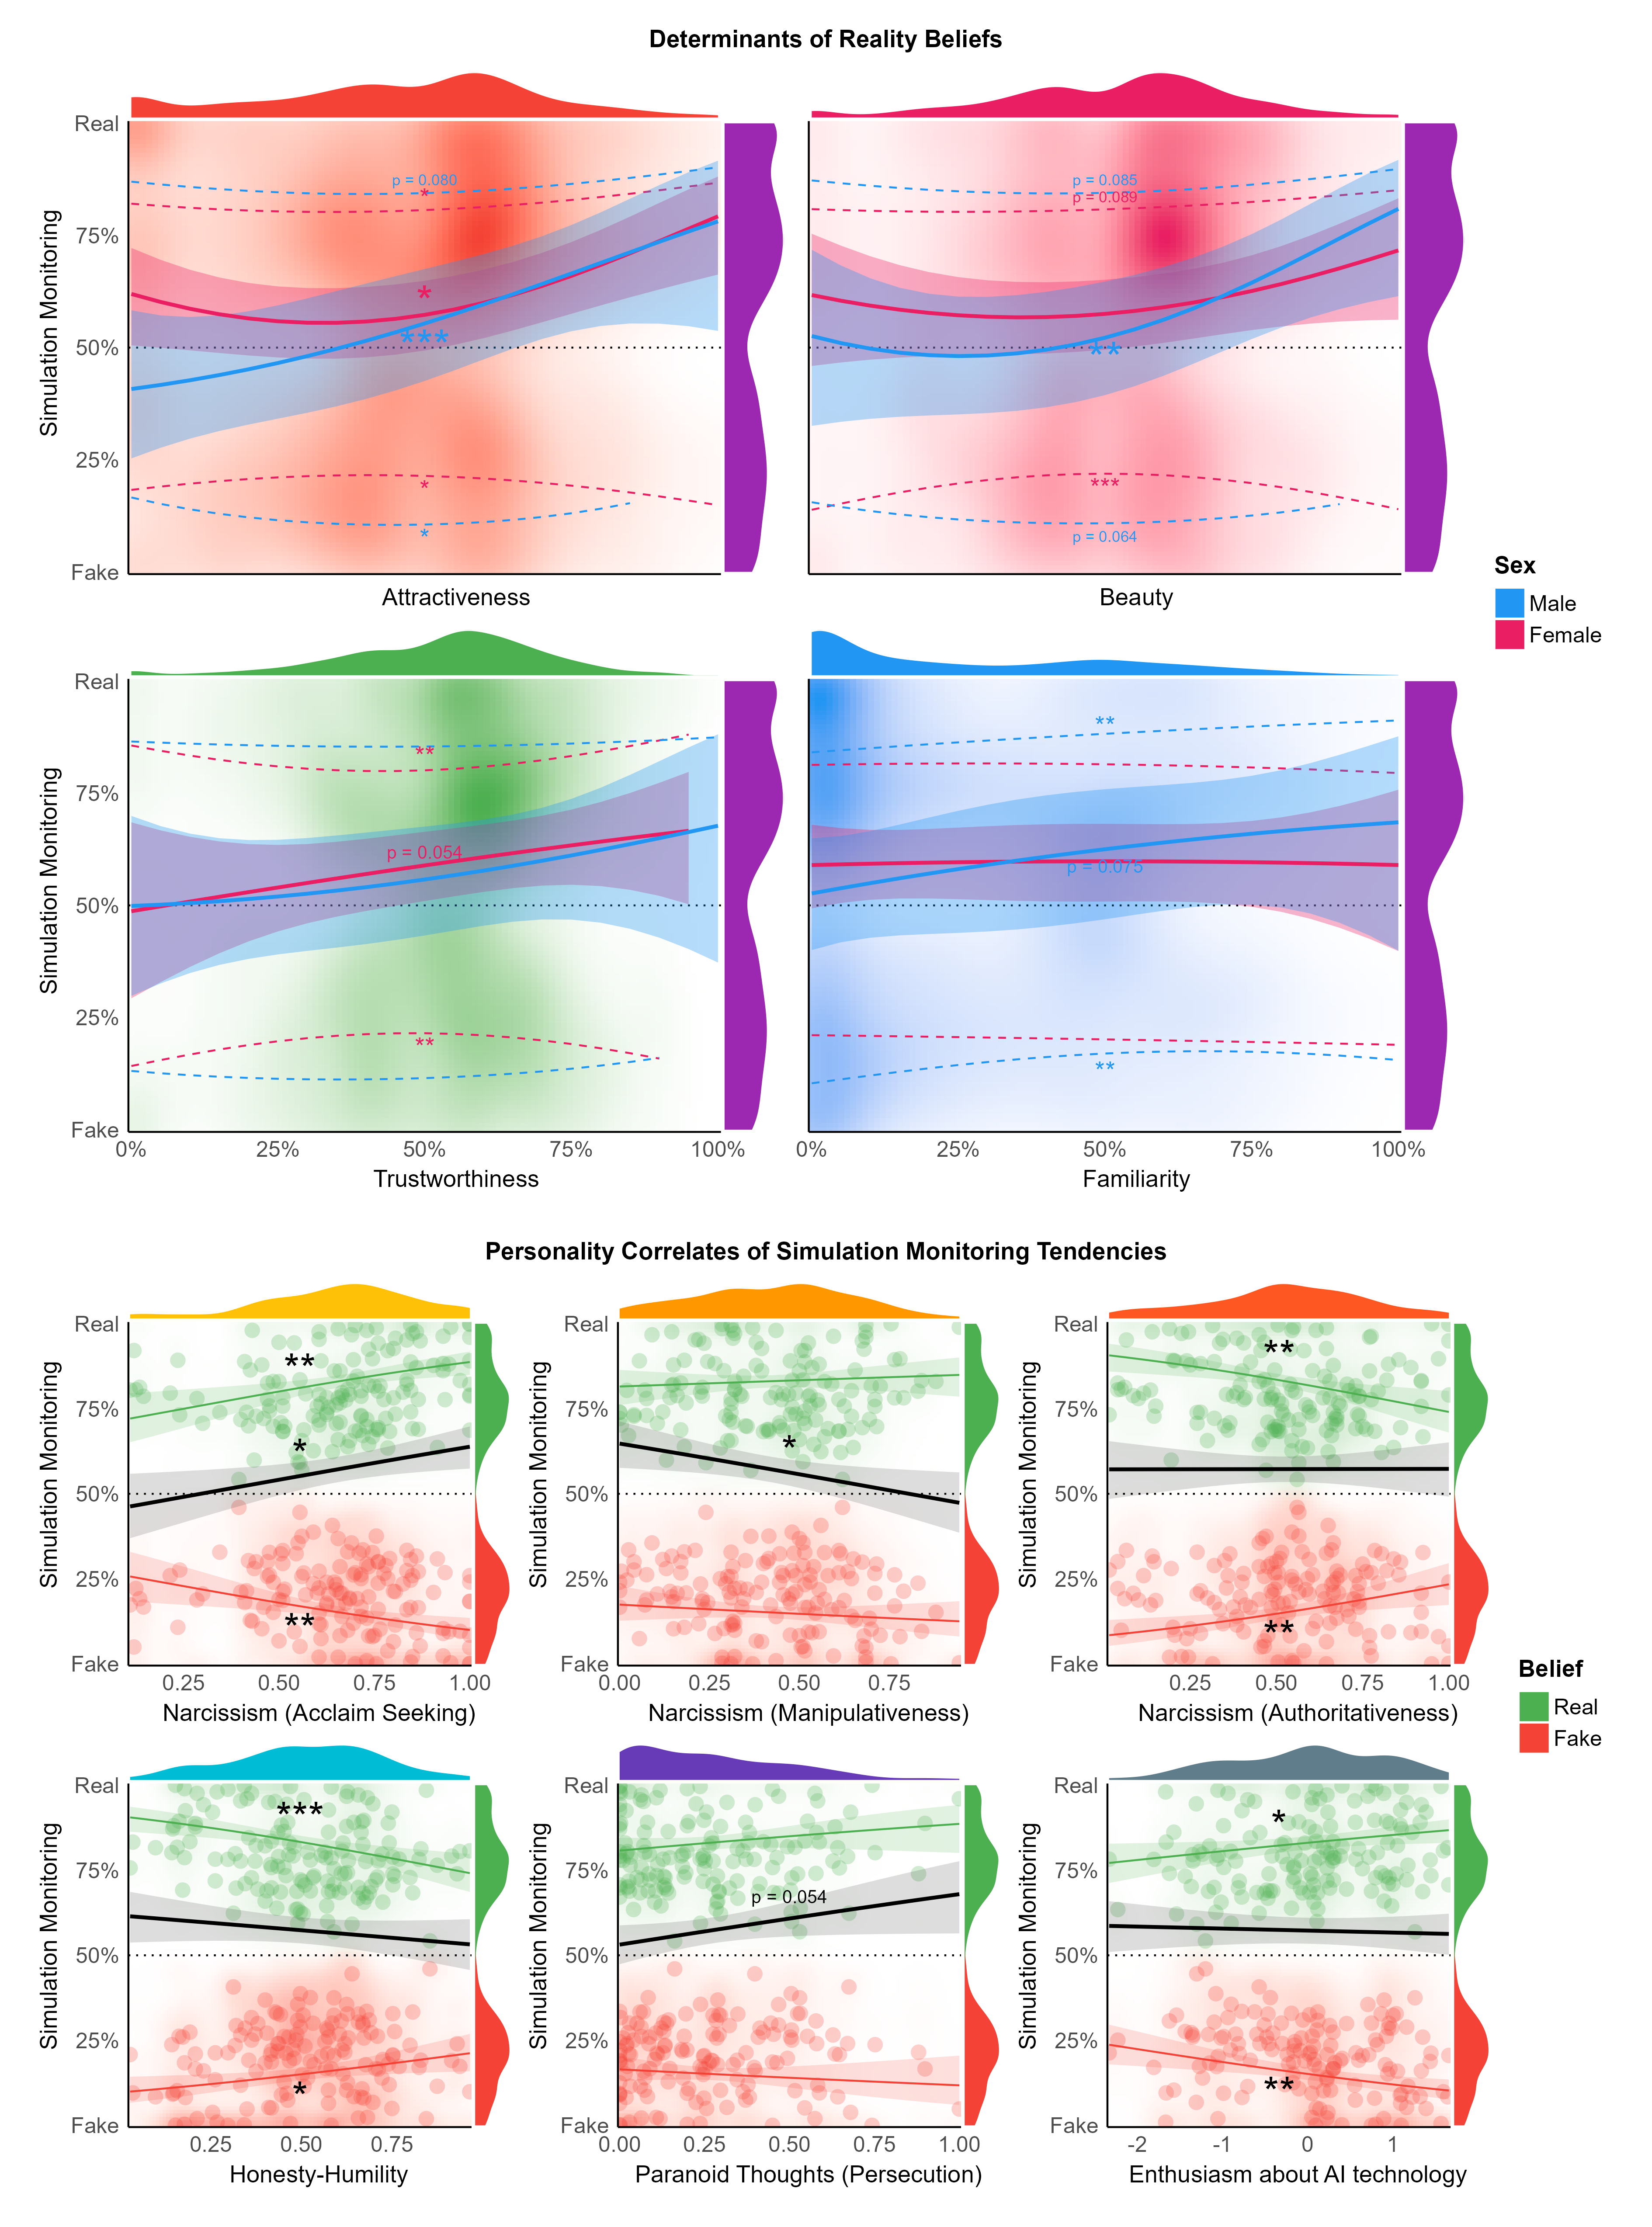
\includegraphics[width=1\linewidth]{../figures/Figure2} \caption{Top part shows blabla.}\label{fig:unnamed-chunk-3}
\end{figure}

\hypertarget{methods}{%
\subsection{Methods}\label{methods}}

\hypertarget{procedure}{%
\subsubsection{Procedure}\label{procedure}}

\hypertarget{participants}{%
\subsubsection{Participants}\label{participants}}

\hypertarget{results}{%
\subsection{Results}\label{results}}

\hypertarget{discussion}{%
\subsection{Discussion}\label{discussion}}

\hypertarget{acknowledgments}{%
\section{Acknowledgments}\label{acknowledgments}}

We would like to thank STUDENT NAME for his contribution.

\newpage

\hypertarget{references}{%
\section{References}\label{references}}

\hypertarget{refs}{}
\begin{CSLReferences}{0}{0}
\end{CSLReferences}


\clearpage
\renewcommand{\listfigurename}{Figure captions}


\end{document}
